\documentclass[a4paper]{article}
\usepackage[dutch]{babel}
\usepackage{mathtools}
\usepackage{listings}
\usepackage{graphicx}

\lstset{language=Python}

\begin{document}
\title{Hamming-code in Python 3.6}
\author{Robin van de Griend, Thomas Koopman, Tim Waroux}
\maketitle

\section{Taakverdeling}
Voor het maken van het algoritme hadden we niet echt een taakverdeling gemaakt. Naarmate we bezig waren kwamen we er wel achter dat het handig was dat Robin bleef werken aan het strconv algoritme, en dat Thomas en Tim bezig waren met de andere onderdelen van de code, en hebben samen vooral veel bugs uit het systeem gehaald. We hadden daarentegen de taken voor het schrijven van het verslag wel verdeeld. Robin heeft zich bezig gehouden met de mogelijke verbeterpunten, Thomas heeft zich bezig gehouden met de complexiteit van de algoritmen en functies. Terwijl Tim de opbouw en het ontwerp van de code geschreven heeft. We hadden bovendien afgesproken dat we alles om en nabij 19 juni 2017 af wilde hebben en dit is voor de code grotendeels gelukt en ook had iedereen toen zijn stukje geschreven voor het verslag. Hierna konden we de feedback die Matthijs ons gegeven heeft op onze code nog verwerken.

\section{Wat is een Hamming-code?}
In de codeertheorie houdt men zich bezig met het vertalen van informatie naar een formelere vorm. Hierdoor wil men voorkomen dat, door een toegevoegde waarde te cree\"eren, de informatie afgeschermt is voor ongewenste toegang of bijvoorbeeld de informatie te beschermen tegen transmissies, denk hierbij bijvoorbeeld aan het opslaan van data op je computer, of het gebruik van data in het RAM-geheugen. Een Hamming-code wordt gebruikt om informatie te bescheremen tegen foutjes die op kunnen treden bij deze soorten transmissie. Hierbij kunnen we onderscheid maken tussen foutdetectie en foutcorrectie. Hamming-codes zijn in beide gebieden actief. Onze code, waar verder over geschreven wordt in dit verslag, maakt gebruik van de foutcorrectie eigenschap van een Hamming-code. Hamming-codes worden gezien als de grondleggers van de codeertheorie, zonder deze theorie zouden de computersystemen die wij nu betrouwbaar achten, een stuk minder betrouwbaar zijn.

\subsection{Hoe werkt een Hamming-code?}
Dit leggen we uit aan de hand van een voorbeeld. Namelijk onze (7,4) Hamming-code.
We gebruiken databits met lengte 4, vandaar de 4 in de naam Hamming-code(7,4). We gaan nu 7-4 = 3 pariteitsbits toevoegen. Deze pariteitbits zitten op plekken die machten zijn van twee. Dus in dit geval op, $2^0$ = 1, $2^1$ = 2, $2^2$ = 4. Elke pariteits bit rekent de pariteit uit voor bits in het woord, de positie waarop de pariteitsbit zit bepaald voor welke bits van het woord hij dit doet. Pariteitsbit 1 checkt 1 bit, slaat er dan 1 over, checkt 1, etc. Dus vormt de rij (1,3,5,7). Pariteitsbit 2 checkt 2 bits, slaat er dan 2 over, checkt er dan 2, etc. Dus vormt de rij (2,3,6,7), en dit gaat zo verder voor alle pariteitsbits. Een pariteitsbit neem de waarde 1 aan als er een oneven aantal enen staan in deze rij, en neemt 0 aan als er een even aantal enen staan. Door te kijken of de pariteitsbits voldoen aan deze eis kunnen we eventuele 1 bits fouten vinden en verbeteren. Een voorbeeld met (1,0,0,0). We schrijven eerst de vector met alle bits op de goeie plek: (p$_1$,p$_2$,1,p$_4$,0,0,0), en dan passen we alles toe wat hierboven beschreven staat. Voor p$_1$ checken we dus de rij die hierboven beschreven staat: (p$_1$,1,0,0). Dit is een oneven aantal 1-en dus schrijven we p$_1$ = 1. Voor p$_2$ volgt het zelfde principe: (p$_2$,1,0,0), dus p$_2$ = 1. Voor p$_4$ volgt (p$_4$,0,0,0), dus p$_4$ = 0. Oftewel deze kolomvector wordt: (1,1,1,0,0,0,0).

\subsection{Hamming-code met matrixvermenigvuldiging}
Hier nemen we ook weer onze (7,4) Hamming-code als voorbeeld. Onze Hamming-code berust op matrixvermenigvulding. Daarbij gebruiken we twee matrices, namelijk de Codeermatrix, ook wel de getransponeerde van de \\
Generatormatrix:
$\begin{pmatrix}
1&0&0&0 \\
0&1&0&0 \\
0&0&1&0 \\
0&0&0&1 \\
1&1&0&1 \\
1&0&1&1 \\
0&1&1&1
\end{pmatrix}
$\\
Merk op dat deze matrix kolommen heeft van lengte 7, daar komt de 7 vandaan in de naam. Bovendien betekent dit dus ook, zoals we in de vorige sectie gezien hebben, dat er 3 pariteitsbits worden toegevoegd. Naast deze matrix hebben we ook nog de decodeermatrix, ook wel de Pariteitscheckmatrix:
$\begin{pmatrix}
1&0&1&0&1&0&1 \\
0&1&1&0&0&1&1 \\
0&0&0&1&1&1&1

\end{pmatrix}
$\\ 
We gebruiken ook hier weer een 4 bitdatawoord.
Als we het 4 bit datawoord vermenigvuldigen met de Generatormatrix krijgen we dus het datawoord met pariteit. Als voorbeeld gebruiken we de kolomvector (1,1,0,0).\\
$\begin{pmatrix}
1&0&0&0 \\
0&1&0&0 \\
0&0&1&0 \\
0&0&0&1 \\
1&1&0&1 \\
1&0&1&1 \\
0&1&1&1
\end{pmatrix}
$
$\begin{pmatrix}
1\\1\\0\\0
\end{pmatrix}
$
= $\begin{pmatrix}
0\\1\\1\\1\\1\\0\\0
\end{pmatrix}
$
\\Als we het 4 bit datawoord, met pariteit, vermenigvuldigen met de Pariteitscheckmatrix komt er, weer modulo 2 rekenend, de nulvector uit als er geen fout in zit. Zit er wel een fout in dat komt er een vector uit die aangeeft op welke plek de fout zit. Hieronder volgt het voorbeeld met de vector (0,1,1,1,1,0,0), oftewel de vector (1,1,0,0) waaraan we pariteit hebben toegevoegd.\\
$\begin{pmatrix}
1&0&1&0&1&0&1 \\
0&1&1&0&0&1&1 \\
0&0&0&1&1&1&1

\end{pmatrix}
$
$
\begin{pmatrix}
0\\1\\1\\1\\1\\0\\0
\end{pmatrix}
$
= $\begin{pmatrix}
	0\\0\\0
\end{pmatrix}
$, we zien dus dat hier geen fout in zit.
\\ Voegen we nu een fout toe op de eerste plek in de vector, dan krijgen we:\\
 $\begin{pmatrix}
1&0&1&0&1&0&1 \\
0&1&1&0&0&1&1 \\
0&0&0&1&1&1&1

\end{pmatrix}
$
$
\begin{pmatrix}
1\\1\\1\\1\\1\\0\\0
\end{pmatrix}
$
= $\begin{pmatrix}
1\\0\\0
\end{pmatrix}
$\\
Nu zoeken we de kolomvector (1,0,0) op in de Pariteitscheckmatrix, we zien dat deze in de eerste kolom staat dus volgt hieruit dat er een fout zit op de eerste bitplek. Merk op dat als er dus op 2 verschillende plekken fouten ontstaan we deze alleen maar kunnen detecteren en niet kunnen herstellen!
\section{Ontwerp van de code}
We hebben er voor gekozen om gebruik te maken van verschillende modules, we hebben voor belangrijke functies een apart bestand aangemaakt. Dit is beter voor de leesbaarheid en maakt het makkelijker om te werken in de code. Hieronder volgt een toelichting voor de verschillende modules.

\subsection{matrix.py}
	Om te beginnen met het programmeren van de Hammingcode, hebben we ervoor gekozen om eerst een klasse Matrix te definieren. Dit staat eveneens aangegeven in de opdracht die we gevolgd hebben. Hier is al onze code opgebasseerd omdat we bij onze hammingcode gebruik maken van de matrixvermenigvuldiging.

\subsection{strconv.py}
	Onze stringconvert bestand is van essentieel belang voor onze hammingcode. De functies die gedefinieerd staan in stringconvert zorgen ervoor dat een string, met name de teskt die mensen willen versturen of opslaan, omzet naar een lijst met matrices. Hierdoor kunnen we ze gebruiken in het Hamming bestand, waar onze Hammingcode wordt uitgevoerd.

\subsection{hamming74 \& hamming84.py}
	In deze bestanden staan onze algoritmen voor de hammingcode. Hamming84.py is feitelijk een copy van hamming74.py, echter zijn alleen de generatormatrix en de pariteitscheck matrix aangepast. Beide bestanden zijn afhankelijk van de variabele 'length'. Hier door weet het algoritme of het om de (8,4) of om de (7,4) hammingcode gaat. In dit bestand staan verder de functies waarmee we pariteit kunnen toevoegen aan bits, eventuele 1 bits fouten kunnen vinden en als deze er zijn herstellen, verder is er nog een functie waarmee we de pariteit van de bits kunnen verwijderen om later in interface.py de string van 1-en 0'en terug te vertalen naar iets wat wij kunnen lezen.

\subsection{errormaker.py}
	Dit is een klein bestand waarin we 2 functies hebben gedefinieerd: Errormaker, de functie waarmee we random 1 bits fouten kunnen maken in een lijst met vectoren waar pariteitbits aaantoegevoegd zijn, en Errormakerstring de functie waar we in een string van 1-en 0'en random 1 bits fouten kunnen maken.	

\subsection{interface.py}
	Dit is het bestand dat de gebruiker van ons programma moet opstarten. In dit bestand komen alle functies van de andere bestanden samen en worden ze samengebruikt om berichten te encoderen en decoderen, en bij het decoderen eventueel een aantal 1 bits fouten toe tevoegen om te laten zien dat het programma deze fouten kan herstellen.
	
\section{Opbouw van de code}
Onze code is opgebouwd uit een aantal modules die gebruikt worden in verschillende algoritmen. Onze belangrijkste module is de class Matrix die gedefinieerd staat in matrix.py, deze module wordt in alle andere algoritmen gebruikt. Daarnaast is onze code opgebouwd uit de hammingcode zelf, waarbij er geen wezenlijk verschil is tussen (7,4) en (8,4) los van de matrices die er in gedefinieerd zijn. Daarnaast is er nog strconv.py en errormaker.py. Al de boven genoemde bestanden worden gebruikt in interface.py. Daar staat het algoritme waar eigenlijk alleen maar de functies worden aangeroepen die van belang zijn voor de output en staan in de andere bestanden.

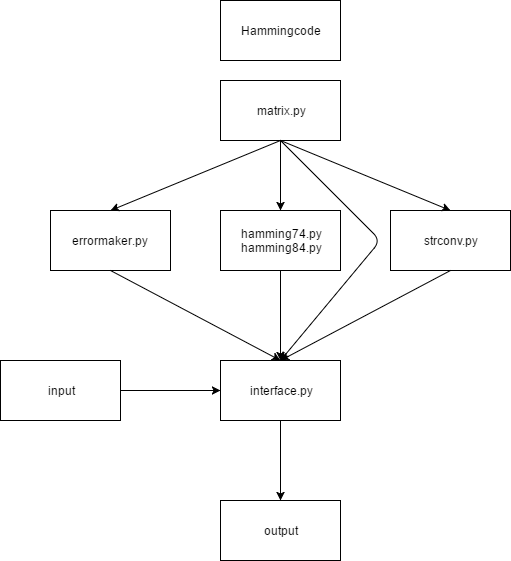
\includegraphics[height=12cm]{diagram}
\\
\\
Om bovenstaande tekst wat toe te lichten hebben we een flowchart gemaakt van hoe de bestanden met elkaar verbonden zijn. Interface.py krijgt een input en gebruikt daar alle bestanden voor die een pijltje hebben dat naar interface.py wijst. interface.py gebruikt dan deze input en zet het dan om in de gevraagde output. Let wel op dat input en output geen aparte bestanden zijn maar zich in wezen in interface.py bevinden


\section{Complexiteit}
We drukken de complexiteit uit in de lengte van de boodschap \(n\). Of dit in bits of in tekens of in matrices is, maakt niet uit omdat elk teken 8 bits is, en elk teken 1 matrix is. Dus in grote O notatie maakt dit niet uit.

encodeentiremessage is O(n) want message is een lijst van n matrices (elk karakter is 1 matrix), en je loopt 1 keer door de lijst heen, en voert elke keer een constant aantal operaties uit. Een lege lijst new\_message maken en dit returnen hangt niet van n af en is dus constant.

Alles behalve de functies $decoderen$, $encoderen$, $binary\_to\_codelist$, $codelist\_to\_str$, $str\_to\_codelist$, $encodeentiremessage$, $repairentiremessage$ en $destroyallparitybits$ krijgen geen boodschap of lijst met matrices als input, dus die zijn O(1). 

\subsection{destroyallparitybits}

Er wordt een lokale variabele new\_message gemaakt, dit is O(n). De lijst parity bits en new\_message ook. Dus dit algoritme is O(n).

\subsection{encodeentiremessage}

Dit is ook O(n), analoog aan $destroyallparitybits$.

\subsection{repairentiremessage}

Dit is ook O(n), analoog aan $destroyallparitybits$.

\subsection{binary\_to\_codelist}

De lijst bytelist aanmaken is O(n). Daarna komen er twee loops die O(n) keer worden aangeroepen, waarin O(1) dingen gebeuren, dus dit algoritme is O(n).

\subsection{codelist\_to\_str}

De lijst codepairs aanmaken is O(n), de loop eronder wordt $n$ keer uitgevoerd en er gebeuren O(1) dingen in, dus dit is ook O(n). Dit algoritme is dus O(n).

\subsection{str\_to\_codelist}

Er wordt een bytearray gemaakt en opgeslagen, dit is O(n). Dan is er een loop van lengte $n$ waarin allerlei O(1) operaties worden uitgevoerd. Dit is dus een O(n) algorithme. 


Het geval destroyallparitybits is analoog.

\subsection{encoderen}

Alles is O(1) behalve het aanroepen van str\_to\_codelist en encodeentiremessage, die beiden O(n) zijn, dus dit is O(n).

\subsection{decoderen}

Alles is O(1) behalve het aanroepen van binary\_to\_codelist, repairentiremessage, destroyallparitybits en codelist\_to\_str die allen O(n) zijn, dus dit is O(n).




\section{Verbeterpunten en mogelijke uitbreidingen van de code}
De Matrix klasse hebben is een zelfgeschreven library waarvan de interface nog verbetert zou kunnen worden. Zo komt het vaak voor in de code waar we lijst-operaties willen uitvoeren op vectoren, een matrix met 1 rij. Op het moment moet je dan de waarden van de matrix opvragen en opslaan als lijst om vervolgens weer opnieuw een matrix aan te moeten maken met de nieuwe lijst van waarden. Zoals de interface nu is geschreven ontstaan er situaties als deze:
\begin{lstlisting}
	code_pairs = [(codelist[i].values[0], 
		codelist[i + 1].values[0]) 
		for i in range(0, len(codelist) - 1, 2)]
\end{lstlisting}
Dit is een stukje code uit \texttt{strconv.py} waar we een lijst van matrices \texttt{codelist} uit willen pakken en voor elke matrix een lijst-operatie willen uitvoeren. In feite zijn maken we hier nergens gebruik van de Matrix-klasse maar toch staan onze codes opgeslagen in een matrix omdat we matrix-vermenigvuldiging gebruiken in het hamming-algoritme.

Veel beter zou het zijn om een externe library te gebruiken als numpy, waar matrices en vectoren een intuïtieve interface hebben. Ook is de code sneller omdat veel rekenintensieve functies in C zijn geïmplementeerd. Verder zou functionaliteit in \texttt{strconv.py} in de Matrix-klasse gebouwd kunnen worden. Het gaat immers om het omzetten van matrices naar andere objecttypes of vice versa. Op die manier houden we functionaliteit die bij matrices hoort bij elkaar.

We zouden Hamming-codes algemener kunnen implementeren. Een Hamming-code wordt volledig vastgelegd door zijn controle-matrix, de genererende matrix kan immers hieruit bepaald worden. We zouden een code kunnen schrijven die voor algemene (n,k,d)-Hamming codes de \(n \times d\) controle-matrix maakt en hieruit de genererende matrix vindt. Op deze manier hoeven we geen matrices expliciet te definiëren en kunnen we ze "as needed" genereren.

Wat ook verbeterd kan worden is het feit dat we nu 2 vrijwel dezelfde bestanden hebben, hamming74.py en hamming84.py. Het enige verschil zoals al aangekaart in het verslag zijn de gedefinieerde matrices. Dit zou misschien wel in \'e\'en bestand kunnen. Want alle functies in beide bestanden zijn alleen nog afhankelijk van het aantal rijen in de generator matrix. Daarnaast belemmerd str\_to\_codelist in strconv.py ons nog om het algoritme te gebruiken bij hammingcode's waarbij het bit-woord ongelijk is aan 4. Dit zouden we kunnen verbeteren door een algemenere functie te maken die afhankelijk van het aantal kolommen in de generatormatrix het bit-datawoord in de codelist zet zodat we daar dan pariteit aan toe kunnen voegen. Waardoor onze Hamming-code gedefinieerd is voor elke lengte van het bit-datawoord.

\section{De Gebruikershandleiding}
Om ons programma te kunnen gebruiken dient u, het bestand: interface.py te openen. Merk op dat u hiervoor wel python 3.6.1 op uw computer ge\"instaleerd moet hebben. Heeft u dit niet dan gaat u naar www.python.org, de website van de programeertaal, en download u daar de versie 3.6.1.\\
\\
Als u nu interface.py heeft opgestart volgt u de instructies op het scherm. Wilt u een bericht klaar maken voor transmissie? Dan gebruikt u encoding.\\
\\
Heeft een bericht ontvangen, dan gebruikt u decoding en kiest u 'nee' als er wordt gevraagd of u random 1 bits fouten wilt toevoegen, deze functie is alleen toegevoegd zodat u makkelijk kan checken of het programma daadwerkelijk wel werkt. Anders kan dit ten koste gaan van de correctheid van het bericht dat u als output krijgt.\\
\\
Het volgende is bedoelt voor de meer ervaren gebruiker:\\
Er zijn enkele functies die niet gebruikt worden in de code maar, die we wel hebben toegevoegd. codelist\_to\_binary in strconv.py en errormakerlist in errormaker.py. U kunt deze functies gebruiken wanneer u wilt, maar dan moeten er wel kleine aanpassingen in de code worden aangebracht. Deze functies zijn echter op dit moment niet nodig om de code te laten functioneren.
\end{document}
